\documentclass[article]{beamer}
\usetheme{Warsaw}
\setbeamertemplate{footline}[frame number]


\usefonttheme[]{serif}
\usepackage{amsmath, latexsym, color, graphicx, amssymb, bm, here}
\usepackage{epsf, epsfig, pifont,tikz,subfigure}
\usepackage{graphics, calrsfs}
\usepackage{times}
\usepackage{fancybox,calc}
\usepackage{palatino,mathpazo}
\usepackage{amsfonts}
%\usepackage{wrapfig}
%\usepackage{multicol}
\usepackage{sidecap}
\usepackage{movie15}
\usepackage{hyperref}
\usepackage{handoutWithNotes}
\usepackage{pgf,pgfarrows,pgfnodes}



\title{Advanced Beamer Techniques}
\author{Stephan Henning}
\institute{Auburn University}
\date{\scriptsize{\today}}



\AtBeginSection[]
{
  \begin{frame}{Outline}
    \tableofcontents[currentsection]
  \end{frame}
}


\begin{document}

%%%%%%%%%%%%%%%%%%%%%%%%%%%%%%Frame 1

\maketitle


%%%%%%%%%%%%%%%%%%%%%%%%%%%%%%Frame 2
\begin{frame}
\frametitle{Outline}
\tableofcontents
\end{frame}


%%%%%%%%%%%%%%%%%%%%%%%%%%%%%%Frame 3
\section{Transitions}
\subsection{Overview}

%%%%%%%%%%%%%%%%%%%%%%%%%%%%%%Frame 4
\begin{frame}[fragile]
\frametitle{Transitions}
\framesubtitle{What are they?}

Simply, an animation used to 'enhance' the movement from the current frame to the next.

\end{frame}

%%%%%%%%%%%%%%%%%%%%%%%%%%%%%%Frame 99
\begin{frame}[fragile]
\frametitle{Transitions}
\framesubtitle{Slide vs Frame}

First we need to define the difference between a slide and a frame. With beamer, frames are created with the \verb|\begin{frame}| command. Slides are then created within that frame when using overlays. Transitions are used for frames, but can be applied to overlays if desired (but please don't).

\end{frame}


%%%%%%%%%%%%%%%%%%%%%%%%%%%%%%Frame 99
\subsection{Frames}

%%%%%%%%%%%%%%%%%%%%%%%%%%%%%%Frame 99
\begin{frame}[fragile]
\frametitle{Transitions}
\framesubtitle{Example-Frames}


\begin{block}{Ready. Set. Go!}
How much wood could a Woodchuck chuck if a Woodchuck could chuck wood?
\end{block}
\end{frame}

%%%%%%%%%%%%%%%%%%%%%%%%%%%%%%Frame 99
\begin{frame}[fragile]
\frametitle{Transitions}
\framesubtitle{Example-Frame cont.}

\transboxin
\begin{block}{Answer:}
\hspace*{40pt} 42
\end{block}

\end{frame}


%%%%%%%%%%%%%%%%%%%%%%%%%%%%%%Frame 99
\begin{frame}[fragile]
\frametitle{Transitions}
\framesubtitle{Example Syntax}

Placed on the frame to be revealed by the transition.

\begin{block}{Rather simple}
\begin{verbatim}
\transboxin
\begin{block}{Answer:}
\hspace*{40pt} 42
\end{block}
\end{verbatim}
\end{block}
\end{frame}

%%%%%%%%%%%%%%%%%%%%%%%%%%%%%%Frame 99
\begin{frame}[fragile]
\frametitle{Transitions}
\framesubtitle{Available transitions}


\tiny{\begin{verbatim}
\transblindshorizontal  Horizontal blinds pulled away
\transblindsvertical    Vertical blinds pulled away
\transboxin             Move to center from all sides
\transboxout            Move to all sides from center
\transdissolve          Slowly dissolve what was shown before
\transglitter           Glitter sweeps in specified direction
\transslipverticalin    Sweeps two vertical lines in
\transslipverticalout   Sweeps two vertical lines out
\transhorizontalin      Sweeps two horizontal lines in
\transhorizontalout     Sweeps two horizontal lines out
\transwipe              Sweeps single line in specified direction
\transduration{2}       Show slide specified number of seconds
\end{verbatim}}

\end{frame}

%%%%%%%%%%%%%%%%%%%%%%%%%%%%%%Frame 99
\subsection{Overlays}

%%%%%%%%%%%%%%%%%%%%%%%%%%%%%%Frame 99
\begin{frame}[fragile]
\frametitle{Transitions}
\framesubtitle{Overlays}
\setbeamercovered{dynamic}

\transboxin<1>
\transglitter<2>
\transwipe<3>
\begin{itemize}
\item  It's an overlay!\\ \pause
\item  And another, oh ya!\\ \pause
\item  And a third! Wow, my lucky day!\\ 
\end{itemize}
\end{frame}


%%%%%%%%%%%%%%%%%%%%%%%%%%%%%%Frame 99
\begin{frame}[fragile]
\frametitle{Transitions}
\framesubtitle{Overlay Syntax}

\begin{block}{Syntax}
\begin{verbatim}
\transboxin<1>
\transglitter<2>
\transwipe<3>
\begin{itemize}
\item  It's an overlay!\\ \pause
\item  And another, oh ya!\\ \pause
\item  And a third! Wow, my lucky day!\\ 
\end{itemize}
\end{verbatim}

\end{block}

\end{frame}


%%%%%%%%%%%%%%%%%%%%%%%%%%%%%%Frame 99
\section{Multimedia}
\subsection{movie15}
%%%%%%%%%%%%%%%%%%%%%%%%%%%%%%Frame 99
\begin{frame}[fragile]
\frametitle{Movie Files}
\framesubtitle{movie15 package}
movie15.sty should be included with the MiKTeX package.

\begin{verbatim}
\usepackage{movie15}
\usepackage{hyperref}
\end{verbatim}

\end{frame}

%%%%%%%%%%%%%%%%%%%%%%%%%%%%%%Frame 99
\subsection{Using movie15}

\begin{frame}[fragile]
\frametitle{Movie Files}
\framesubtitle{.mp4}

\begin{figure}[ht]
\includemovie[
  poster,
  text={\small(Loading...)}
]{6cm}{6cm}{Circle-m-increase3.mp4}
\end{figure}
\end{frame}


%%%%%%%%%%%%%%%%%%%%%%%%%%%%%%Frame 99
\begin{frame}[fragile]
\frametitle{Movie Files}
\framesubtitle{.mp4 syntax}

\begin{block}{Relatively simple}

\begin{verbatim}
\begin{figure}[ht]
\includemovie[
  poster,
  text={\small(Loading...)}
]{6cm}{6cm}{Circle-m-increase3.mp4}
\end{figure}
\end{verbatim}

\end{block}

\end{frame}


%%%%%%%%%%%%%%%%%%%%%%%%%%%%%%Frame 99
\begin{frame}[fragile]
\frametitle{Movie Files}
\framesubtitle{Flash}

\begin{figure}[h!]
\includemovie[
  poster=pcb.jpg,
  text={\Large\bf\color{white}{Start}\hspace*{40pt}}
]{6cm}{6cm}{blendone.swf}
\end{figure}
\end{frame}


%%%%%%%%%%%%%%%%%%%%%%%%%%%%%%Frame 99
\begin{frame}[fragile]
\frametitle{Movie Files}
\framesubtitle{Flash syntax}

\begin{block}{Basically the same.}

\footnotesize{\begin{verbatim}
\begin{figure}[h!]
\includemovie[
 poster=pcb.jpg,
 text={\Large\bf\color{white}{Start}\hspace*{40pt}}
]{6cm}{6cm}{blendone.swf}
\end{figure}
\end{verbatim}}
Files and TeX courtesy of http://www.uoregon.edu/~noeckel/PDFmovie.html
\end{block}

\end{frame}

%%%%%%%%%%%%%%%%%%%%%%%%%%%%%%Frame 99
\section{Drawing in Beamer}
\subsection{Intro to pgf}

%%%%%%%%%%%%%%%%%%%%%%%%%%%%%%Frame 99
\begin{frame}[fragile]
\frametitle{pgf package}
\framesubtitle{Overview}

Used to create basic shapes within beamer.
\\[15pt]
Can be used to create tables, graphs, flowcharts and anything that you have the patience to create when you don't have an image to import.
\\[15pt]
pfg package is included with MiKTeX.
\begin{verbatim}
\usepackage{pgf,pgfarrows,pgfnodes}
\end{verbatim}

Please see the following document for more info: 
\tiny{\begin{verbatim}
http://mixing.coas.oregonstate.edu/links/latex_files/pgfuserguide.pdf 

\end{verbatim}}


\end{frame}

%%%%%%%%%%%%%%%%%%%%%%%%%%%%%%Frame 99
\subsection{pgf Examples}

%%%%%%%%%%%%%%%%%%%%%%%%%%%%%%Frame 99
\begin{frame}[fragile]
\frametitle{pgf package}
\framesubtitle{Example1}


\begin{columns}
\column{.2\textwidth}
\begin{block}{Result}
\begin{pgfpicture}{0cm}{0cm}{2cm}{2cm}
% (0cm,0cm) is the lower left corner,
% (5cm,2cm) is the upper right corner.
\pgfrect[stroke]{\pgfpoint{0cm}{0cm}}{\pgfpoint{2cm}{10pt}}
% Paint a rectangle (stroke it, do not fill it)
% The lower left corner is at (0cm,0cm)
% The rectangle is 2cm wide and 10pt high.
\pgfcircle[fill]{\pgfpoint{1cm}{1cm}}{10pt}
% Paint a filled circle
% The center is at (1cm,1cm)
% The radius is 10pt
\end{pgfpicture}
\end{block}
\column{.7\textwidth}
\begin{block}{Syntax}
\tiny{\begin{verbatim}
\begin{pgfpicture}{0cm}{0cm}{5cm}{5cm}
% (0cm,0cm) is the lower left corner,
% (5cm,2cm) is the upper right corner.
\pgfrect[stroke]{\pgfpoint{0cm}{0cm}}{\pgfpoint{2cm}{10pt}}
% Paint a rectangle (stroke it, do not fill it)
% The lower left corner is at (0cm,0cm)
% The rectangle is 2cm wide and 10pt high.
\pgfcircle[fill]{\pgfpoint{3cm}{1cm}}{10pt}
% Paint a filled circle
% The center is at (3cm,1cm)
% The radius is 10pt
\end{pgfpicture}
\end{verbatim}}
\end{block}\end{columns}



\end{frame}

%%%%%%%%%%%%%%%%%%%%%%%%%%%%%%Frame 99
\begin{frame}[fragile]
\frametitle{pgf package}
\framesubtitle{Example2}


\begin{columns}
\column{.2\textwidth}
\begin{block}{Result}
\begin{pgfpicture}{-.2cm}{-.2cm}{2cm}{2cm}
\pgfsetstartarrow{\pgfarrowto}
\pgfsetendarrow{\pgfarrowsingle}
\pgfxycurve(0,0.25)(0.5,0.5)(1,0)(1.5,0.25)\end{pgfpicture}
\end{block}
\column{.7\textwidth}
\begin{block}{Syntax}
\tiny{\begin{verbatim}
\begin{pgfpicture}{.2cm}{.2cm}{5cm}{5cm}
\pgfsetstartarrow{\pgfarrowto}
\pgfsetendarrow{\pgfarrowsingle}
\pgfxycurve(0,0.25)(0.5,0.5)(1,0)(1.5,0.25)
\end{pgfpicture}
\end{verbatim}}
\end{block}\end{columns}



\end{frame}

%%%%%%%%%%%%%%%%%%%%%%%%%%%%%%Frame 99
\begin{frame}[fragile]
\frametitle{pgf package}
\framesubtitle{Example3}

\begin{pgfpicture}{0cm}{0cm}{5cm}{5cm}
\pgfnodebox{Node1}[stroke]{\pgfxy(1,0.5)}{hello}{2pt}{2pt}
\pgfnodebox{Node2}[stroke]{\pgfxy(4,.5)}{world}{2pt}{2pt}
\pgfnodebox{Node3}[stroke]{\pgfxy(7,.5)}{lovely}{2pt}{2pt}
\pgfnodeconncurve{Node1}{Node2}{0}{90}{1cm}{1cm}
\pgfnodeconncurve{Node1}{Node2}{0}{90}{1cm}{1.5cm}
\pgfnodeconncurve{Node1}{Node2}{0}{90}{1cm}{2cm}
\pgfnodeconncurve{Node1}{Node2}{0}{90}{1cm}{2.5cm}
\pgfnodeconncurve{Node2}{Node3}{-10}{80}{1cm}{1cm}
\pgfnodeconncurve{Node2}{Node3}{-20}{70}{1cm}{1cm}
\pgfnodeconncurve{Node2}{Node3}{-30}{60}{1cm}{1cm}
\pgfnodeconncurve{Node2}{Node3}{-40}{50}{1cm}{1cm}
\end{pgfpicture}
\end{frame}



%%%%%%%%%%%%%%%%%%%%%%%%%%%%%%Frame 99
\begin{frame}[fragile]
\frametitle{pgf package}
\framesubtitle{Example3-Syntax}

\footnotesize{\begin{verbatim}
\begin{pgfpicture}{0cm}{0cm}{5cm}{5cm}
\pgfnodebox{Node1}[stroke]{\pgfxy(1,0.5)}{hello}{2pt}{2pt}
\pgfnodebox{Node2}[stroke]{\pgfxy(4,.5)}{world}{2pt}{2pt}
\pgfnodebox{Node3}[stroke]{\pgfxy(7,.5)}{lovely}{2pt}{2pt}
\pgfnodeconncurve{Node1}{Node2}{0}{90}{1cm}{1cm}
\pgfnodeconncurve{Node1}{Node2}{0}{90}{1cm}{1.5cm}
\pgfnodeconncurve{Node1}{Node2}{0}{90}{1cm}{2cm}
\pgfnodeconncurve{Node1}{Node2}{0}{90}{1cm}{2.5cm}
\pgfnodeconncurve{Node2}{Node3}{-10}{80}{1cm}{1cm}
\pgfnodeconncurve{Node2}{Node3}{-20}{70}{1cm}{1cm}
\pgfnodeconncurve{Node2}{Node3}{-30}{60}{1cm}{1cm}
\pgfnodeconncurve{Node2}{Node3}{-40}{50}{1cm}{1cm}
\end{pgfpicture}
\end{verbatim}}
\end{frame}

%%%%%%%%%%%%%%%%%%%%%%%%%%%%%%Frame 99
\begin{frame}[fragile]
\frametitle{pgf package}
\framesubtitle{Example4}

\begin{pgfpicture}{0cm}{0cm}{5cm}{2cm}
\pgfputat{\pgfxy(1,1)}{\pgfbox[center,center]{Hi!}}
% pgfputat places something at a certain position
% pgfbox shows the text �hi!�. The horizontal alignment
% is centered (other options: left, right). The vertical
% alignment is also centered (other options: top, bottom,
% base).
\pgfcircle[stroke]{\pgfxy(1,1)}{0.5cm}
\pgfsetendarrow{\pgfarrowto}
% In the following, all lines will end with an arrow that looks like
% the arrow of TeX�s \to command
\pgfline{\pgfxy(1.5,1)}{\pgfxy(2.2,1)}
\pgfputat{\pgfxy(3,1)}{
\begin{pgfrotateby}{\pgfdegree{30}}
% You can rotate things like this
\pgfbox[center,center]{$\int_0^\infty xdx$}
\end{pgfrotateby}}
\pgfcircle[stroke]{\pgfxy(3,1)}{0.75cm}
\end{pgfpicture}
\end{frame}



%%%%%%%%%%%%%%%%%%%%%%%%%%%%%%Frame 99
\begin{frame}[fragile]
\frametitle{pgf package}
\framesubtitle{Example4-Syntax}

\footnotesize{\begin{verbatim}
\begin{pgfpicture}{0cm}{0cm}{5cm}{2cm}
\pgfputat{\pgfxy(1,1)}{\pgfbox[center,center]{Hi!}}
% pgfputat places something at a certain position
% pgfbox shows the text �hi!�. The horizontal alignment
% is centered (other options: left, right). The vertical
% alignment is also centered (other options: top, bottom,base).
\pgfcircle[stroke]{\pgfxy(1,1)}{0.5cm}
\pgfsetendarrow{\pgfarrowto}
% In the following, all lines will end with an arrow that 
% looks like the arrow of TeX�s \to command
\pgfline{\pgfxy(1.5,1)}{\pgfxy(2.2,1)}
\pgfputat{\pgfxy(3,1)}{
\begin{pgfrotateby}{\pgfdegree{30}}
% You can rotate things like this
\pgfbox[center,center]{$\int_0^\infty xdx$}
\end{pgfrotateby}}
\pgfcircle[stroke]{\pgfxy(3,1)}{0.75cm}
\end{pgfpicture}
\end{verbatim}}
\end{frame}


%%%%%%%%%%%%%%%%%%%%%%%%%%%%%%Frame 99
\section{Handouts}

%%%%%%%%%%%%%%%%%%%%%%%%%%%%%%Frame 99
\begin{frame}[fragile]
\frametitle{Handouts}
\framesubtitle{Printable Handouts}

\begin{block}{Slides + Notes field}
For those times when you actually want to take notes...
\\
\tiny{\begin{verbatim}
\usepackage{handoutWithNotes}
\pgfpagesuselayout{3 on 1 with notes}[a4paper,border shrink=5mm]
Or
\pgfpagesuselayout{1 on 1 with notes landscape}[a4paper,border shrink=5mm]
\end{verbatim}
}

Several options, see http://www.guidodiepen.nl/2009/07/creating-latex-beamer-handouts-with-notes/

\end{block}

\end{frame}

%%%%%%%%%%%%%%%%%%%%%%%%%%%%%%Frame 99
\begin{frame}[fragile]
\frametitle{Handouts}
\framesubtitle{Results}

\begin{figure}
	\centering
		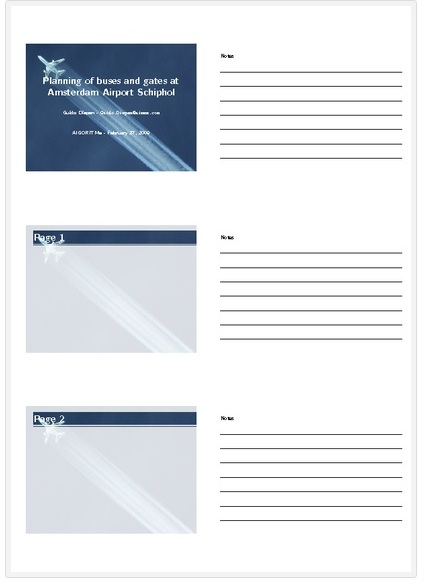
\includegraphics[width=0.4\textwidth]{3n1.jpg}
	\label{fig:3n1}
\end{figure}

\end{frame}

\end{document}